%!TEX root =  main.tex
\section{Experimental evaluation}
\label{sec:experimental-evaluation}

In this section, we present the protocols we compare \libname to (\S\ref{sec:comp}), and
describe the experimental environment (\S\ref{sec:evaluation:setup}).
We conducted three sets of experiments.
In the first set, we seek to understand the effects of message size on \libname (\S\ref{sec:evaluation:micro}).
In the second set, we compare \libname's performance to WBCast's, the best-performing message-passing atomic multicast protocol (\S\ref{sec:evaluation:multicast}).
As we will see, \libname outperforms WBCast.
Even though both protocols are assessed in the same environment, one may wonder whether \libname's advantage is a result of RDMA efficient writes (used by \libname) when compared to RDMA send and receive operations (used by WBCast).
In the third set of experiments, we compare \libname's ``inherent performance'' (i.e., in the absence of contention and queueing effects) to protocols that optimize communication (\S\ref{sec:evaluation:broadcast}).

%\subsection{Evaluation rationale}
\subsection{Competing protocols}
\label{sec:comp}

We experimentally compare \libname to protocols in two categories:
In the first category, we consider high-performance atomic broadcast protocols that rely on RDMA technology (APUS and Mu) or bypass the network stack (Kernel Paxos).
In the second category, we consider a message-passing genuine atomic multicast protocol (WBCast).
In the following, we briefly comment on these protocols and their configuration in the experimental study.
We provide more details about each protocol in Section~\ref{sec:related-work}.

APUS is a general-purpose atomic broadcast protocol that implements Paxos.
As part of the execution, nodes store ordered messages on stable storage (e.g., SSD).
In order to ensure a fair comparison among the various protocols, we configured APUS with a RAM disk storage instead.

Mu \cite{Aguilera2019} implements Protected Memory Paxos.
It was designed to replicate micro services and optimizes atomic broadcast in one important aspect: by co-locating clients and the Paxos's leader on the same host.
As a consequence, the leader can order a broadcast message after one RDMA write delay, needed to place the message in the memory of the followers.
As described in Section~\ref{sec:PMP}, this is enough to ensure that the message is ordered.
Unfortunately, co-locating clients and leaders on the same host is not possible in atomic multicast: the motivation and scalability of atomic multicast stem from the fact that one can create multiple groups, each one operating independently.
We consider Mu in our evaluation since it is the best-performing RDMA-based atomic broadcast protocol.

Kernel Paxos~\cite{esposito2018kernel} is a Multi-Paxos implementation that improves the performance of the original libpaxos library.\footnote{\url{https://bitbucket.org/sciasciad/libpaxos}}
The main idea is to reduce system calls by running Paxos logic in the Linux kernel, bypassing the network stack, and avoiding the TCP/IP stack. 
We used the original code\footnote{\url{https://github.com/esposem/Kernel_Paxos}} and deployed a single group with three replicas.
We compare \libname to Kernel Paxos because both systems avoid the overhead of the communication stack.
%We have chosen such an implementation because we believe that it has similar features to our library, with optimizations for high throughput and low latency.

White-Box Atomic Multicast (WBCast)~\cite{gotsman2019white} is a genuine atomic multicast protocol that delivers exceptional performance, thanks to some algorithmic optimizations.
%can deliver multi-group messages to the leader of each destination group in three communication steps (four communication steps to the remaining replicas in the destination groups).
 WBCast provides a C-language implementation that uses libevent for communication.\footnote{\url{https://github.com/imdea-software/atomic-multicast}}
 We extended the code to include additional statistics information.


\subsection{Environment setup and configuration parameters}
\label{sec:evaluation:setup}

We conducted all experiments using the CloudLab infrastructure~\cite{DuplyakinATC19cloudlab} with two sets of nodes: 
(a) R320 node for the single-group experiments, equipped with one eight-core Xeon E5-2450 processor running at 2.1GHz, 16 GB of main memory, and a Mellanox FDR CX3 NIC; and (b) XL170 nodes for the other experiments, equipped with one ten-core Intel E5-2640v4 processor running at 2.4GHz, 64 GB of main memory, and a Mellanox ConnectX-4 NIC. 
A 10 Gbps network link with around 0.1ms round-trip time connects all nodes running Ubuntu Linux 18.04 with kernel 4.15 an Oracle Java SE Runtime Environment 11. 

In all our experiments, clients and servers are independent processes. 
Clients submit requests in a closed-loop, i.e., each client multicasts a message to servers and waits for a response before multicasting the next message. 
In every protocol, each group has 3 processes with in-memory storage.

%We defined three experimental setups:
%in~\S\ref{sec:evaluation:micro} we deployed \libname with a single group and increasing message size;
%\S\ref{sec:evaluation:broadcast} compares \libname with Kernel Paxos and WBCast in a broadcast (single-group) deployment;
%\S\ref{sec:evaluation:multicast} presents a scenario with eight groups contrasting \libname and WBCast with an increasing number of clients and destination groups.

\begin{figure*}[ht]
  \begin{subfigure}{\columnwidth}
    \advance\leftskip+0.08cm
    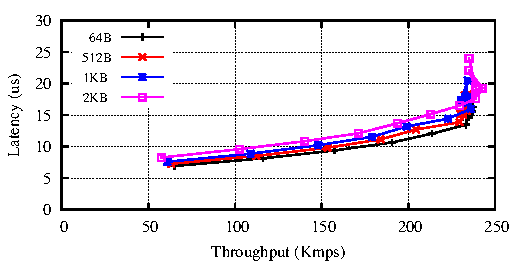
\includegraphics[width=0.97\columnwidth]{figures/benchmark/graphs/figure-performance-vs-size-single-group-up-to-4k}
  \end{subfigure}
  \begin{subfigure}{\columnwidth}
    \advance\leftskip+0.07cm
    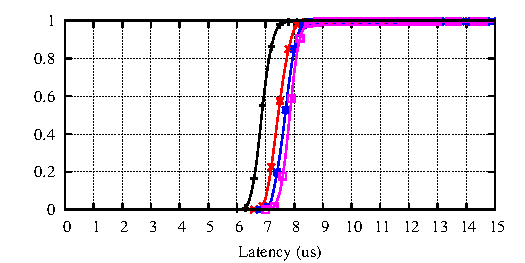
\includegraphics[width=0.96\columnwidth]{figures/benchmark/graphs/figure-performance-vs-size-single-group-cdf-up-to-4k}
  \end{subfigure}
  \begin{subfigure}{\columnwidth}
    \advance\leftskip-0.1cm
    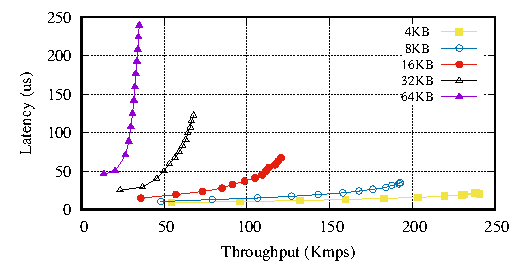
\includegraphics[width=0.99\columnwidth]{figures/benchmark/graphs/figure-performance-vs-size-single-group-from-4k}
  \end{subfigure}
  \begin{subfigure}{\columnwidth}
    \advance\leftskip+0.1cm
    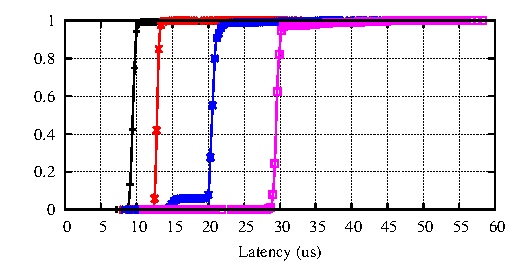
\includegraphics[width=0.96\columnwidth]{figures/benchmark/graphs/figure-performance-vs-size-single-group-cdf-from-4k}
  \end{subfigure}
  \caption{\libname performance with different message sizes: 64B to 2 KB (top) and 4 KB to 32 KB (bottom), throughput versus latency (left) and latency cumulative distribution function for a single client (right).}
  \label{fig:1group_message_size}
\end{figure*}

\subsection{The impact of message size}
\label{sec:evaluation:micro}

In this experiment, conducted on XL170 nodes, we measure \libname throughput and latency for different message sizes.
For each message size, we increase the number of clients until the system is saturated, i.e., throughput stops improving while latency raises.
Figure~\ref{fig:1group_message_size} (left) shows that up to 4KB messages, the impact of message size on the system throughput is negligible, with nearly 250 thousand messages delivered per second. 
As the message size increases past 4KB, the maximum throughput decreases with 35 thousand messages per second for 64KB messages.
The latency cumulative distribution function (CDF) in Figure~\ref{fig:1group_message_size} (right) exhibits minimum latency variation for messages with up to 2KB, around 8 microseconds at $95^{th}$ percentile. At 4KB messages, the latency slightly go up to around 10 microseconds.


\subsection{The performance of atomic multicast}
\label{sec:evaluation:multicast}

The last set of experiments assess \libname behavior in scenarios with up to 8 groups of 3 replicas each, deployed on XL170 machines.
The first experiment comprises executions in which clients send single-group 64-byte messages in setups with 1, 2, 4, and 8 groups.
Figure~\ref{fig:multicast-single-group} (top) shows the aggregated throughput results when the system is saturated. 
\libname outperforms WBCast by a factor of 3.6$\times$ in all configurations.
These results highlight the benefit of genuine atomic multicast algorithms and show that the throughput grows linearly with the number of groups for single-group messages. 
Since groups do not exchange any information when dealing with single-group messages, the latency CDF is the same for a single client, no matter the number of groups in the system, as depicted in Figure~\ref{fig:multicast-single-group} (bottom).

%\begin{figure}[htp!]
%  \begin{subfigure}{\columnwidth}
%    \advance\leftskip-0.25cm
%    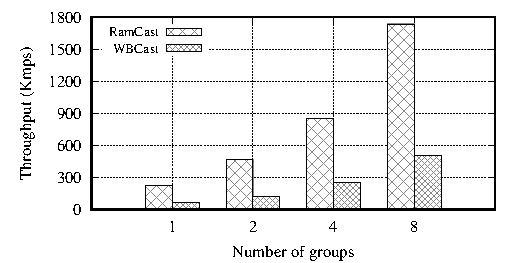
\includegraphics[width=1.01\columnwidth]{figures/benchmark/graphs/figure-genuine-compare-throughput}
%  \end{subfigure}
%  \begin{subfigure}{\columnwidth}
%    \centering
%    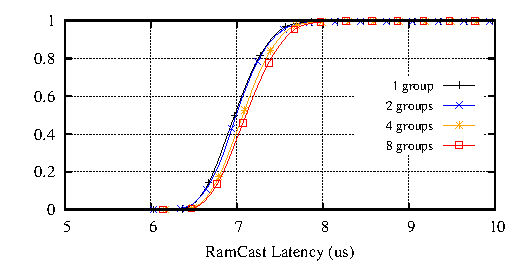
\includegraphics[width=0.95\columnwidth]{figures/benchmark/graphs/figure-genuine-compare-latency-cdf}
%  \end{subfigure}
%  \caption{Performance of atomic multicast when messages are multicast to a single group: throughput (top) and latency cumulative distribution function of a \libname's single client (bottom).}
%  \label{fig:multicast-single-group}
%\end{figure}

The next experiment evaluates the protocols with multi-group messages of 64 bytes addressed to all the groups.
\libname's maximum throughput is greater than WBCast's in every configuration with 233, 145, 80, and 40 thousand messages per second for 1, 2, 4, and 8 destination groups against 63, 50, 35, and 27 thousand for WBCast, as shown in Figure~\ref{fig:multicast-multi-group} (top).
The values correspond to improvements of 3.7$\times$, 2.9$\times$, 2.3$\times$ and 1.5$\times$, respectively.
The difference is even more expressive if we consider the latency for a single client, i.e., when both protocols are contention-free. Figure~\ref{fig:multicast-multi-group} (middle) shows that the latency CDF for \libname with values of 8, 46, 78 and 150~microseconds for 1, 2, 4, and 8 destination groups if we consider the $95^{th}$ percentile. 
The equivalent values for WBCast are 214, 445, 673, and 1055~microseconds, representing 20$\times$ to 7$\times$ slower delivery times when compared to \libname's.

%\begin{figure}[htp!]
%  \begin{subfigure}{\columnwidth}
%    \advance\leftskip-0.1cm
%    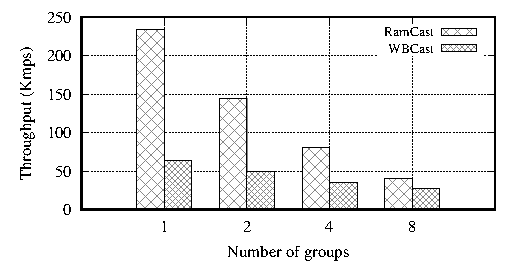
\includegraphics[width=0.99\columnwidth]{figures/benchmark/graphs/figure-multi-dest-compare-throughput}
%  \end{subfigure}
%  \begin{subfigure}{\columnwidth}
%    \centering
%    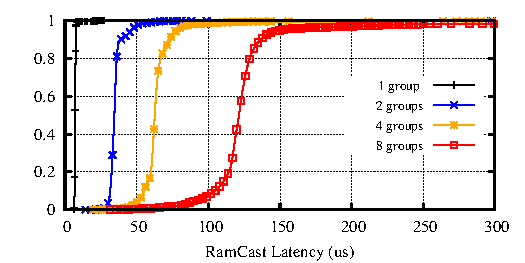
\includegraphics[width=0.95\columnwidth]{figures/benchmark/graphs/figure-multi-dest-compare-latency-cdf-ramcast}
%  \end{subfigure}
%  \begin{subfigure}{\columnwidth}
%    \centering
%    \includegraphics[width=0.95\columnwidth]{figures/benchmark/graphs/figure-multi-dest-compare-latency-cdf-WBCast}
%  \end{subfigure}
%  \caption{Performance comparison of \libname and WBCast for multi-group messages: throughput (top) and latency cumulative distribution function of \libname's (middle) and WBCast's single client (bottom).}
%  \label{fig:multicast-multi-group}
%\end{figure}

\begin{figure*}[ht]
  \begin{subfigure}{\columnwidth}
    \advance\leftskip-0.25cm
    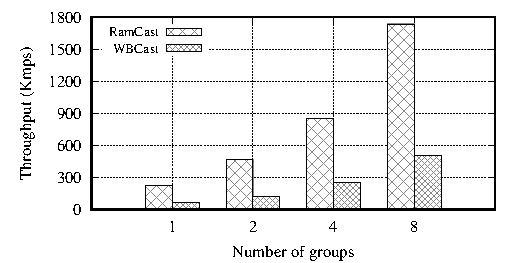
\includegraphics[width=1.01\columnwidth]{figures/benchmark/graphs/figure-genuine-compare-throughput}
  \end{subfigure}
  \begin{subfigure}{\columnwidth}
    \advance\leftskip-0.1cm
    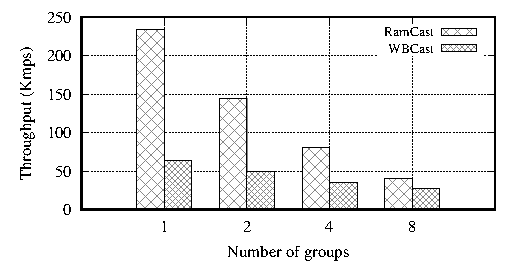
\includegraphics[width=0.99\columnwidth]{figures/benchmark/graphs/figure-multi-dest-compare-throughput}
  \end{subfigure}

  \begin{subfigure}{\columnwidth}
    \centering
    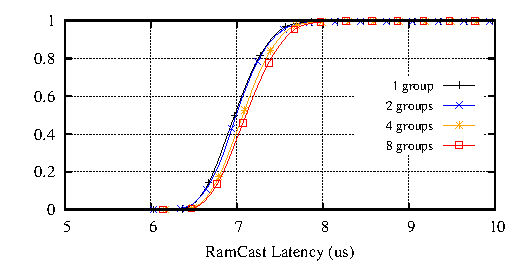
\includegraphics[width=0.95\columnwidth]{figures/benchmark/graphs/figure-genuine-compare-latency-cdf}
  \end{subfigure}
  \begin{subfigure}{\columnwidth}
    \centering
    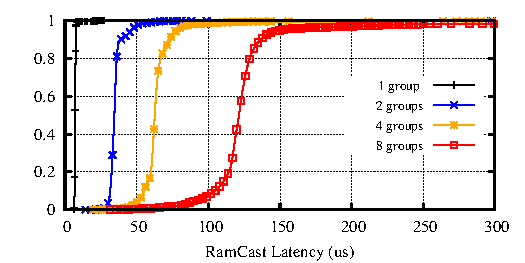
\includegraphics[width=0.95\columnwidth]{figures/benchmark/graphs/figure-multi-dest-compare-latency-cdf-ramcast}
  \end{subfigure}

  \begin{subfigure}{\columnwidth}
    \centering
    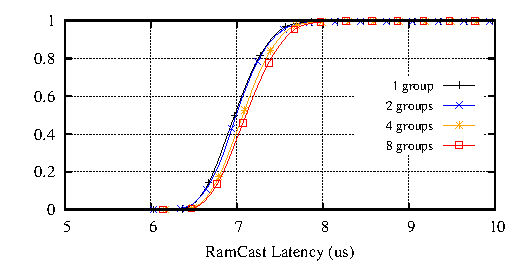
\includegraphics[width=0.95\columnwidth]{figures/benchmark/graphs/figure-genuine-compare-latency-cdf}
  \end{subfigure}
  \begin{subfigure}{\columnwidth}
    \centering
    \includegraphics[width=0.95\columnwidth]{figures/benchmark/graphs/figure-multi-dest-compare-latency-cdf-WBCast}
  \end{subfigure}
  \caption{Performance of atomic multicast when messages are multicast to a single group (graphs on the left) and to all groups (graphs on the right). In each case, we show: throughput (top) and latency cumulative distribution function with one client of \libname (middle) and WBCast (bottom).}
  \label{fig:1group_message_size}
\end{figure*}

\begin{figure}[htp!]
  \begin{subfigure}{\columnwidth}
    \advance\leftskip-0.0cm
    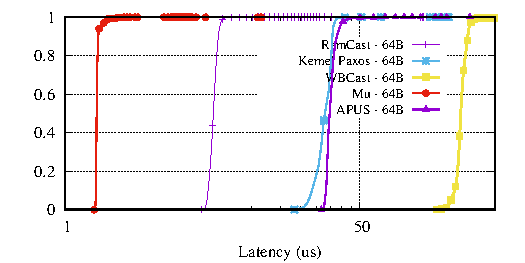
\includegraphics[width=1\columnwidth]{figures/benchmark/graphs/figure-compare-single-group-latency-cdf-64b}
  \end{subfigure}
  \begin{subfigure}{\columnwidth}
    \centering
    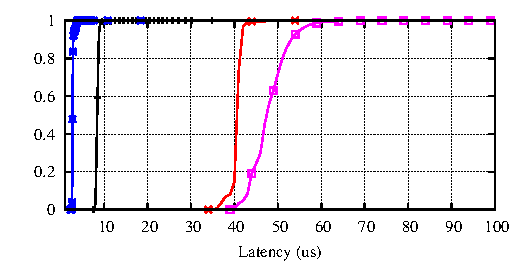
\includegraphics[width=1\columnwidth]{figures/benchmark/graphs/figure-compare-single-group-latency-cdf-1k}
  \end{subfigure}
  \caption{Latency cumulative distribution function for \libname and atomic broadcast protocols with a single client: 64-byte messages (top) and 1K-byte messages (bottom).}
  \label{fig:broadcast}
\end{figure}



\subsection{\libname's inherent performance}
\label{sec:evaluation:broadcast}

This experiment assesses how each protocol behaves in a scenario with a single group of three replicas, and 64-byte and 1-kilobyte messages.
Figure~\ref{fig:broadcast} (top) shows that, for 64-byte messages, \libname outperforms the competitors with approximately 200 thousand messages per second. 
Kernel Paxos comes close with 170 thousand messages per second, while WBCast saturates sooner, with less than 60 thousand messages per second.
For larger messages, \libname kept the same performance, while the other protocols had the throughput reduced by half.
Figure~\ref{fig:broadcast} (bottom) confirms the superior results for \libname. The median latency for WBCast with small messages and a single client is twenty times greater than the same measurement for \libname.


